\subsection{Android}

	Bereits durch die Architektur des Betriebssystems, insbesondere durch die restriktive Rechtevergabe und das Sandboxing, wird versucht, ein möglichst sicheres System bereitzustellen. Ab Android Version 4.3 kommt zusätzlich noch \textit{Security-Enhanced Linux (SELinux)} zum Einsatz. Verschlüsselungen und Signaturen werden Hardwareseitig durch eine \textit{Trusted Execution Environment (TEE)} unterstützt. TEE stellt einen besonders geschützten Bereich auf dem Prozessor dar, auf dem nur berechtige Anwendungen ausgeführt werden können, wie beispielsweiße die Verifikation des Bootmediums und Verschlüsselungsverfahren. Die Implementierung ist dabei Prozessor Hersteller abhängig - auf ARM wird dabei, wie bei iOS, auf \textit{TrustZone}\cite{TEE_ARM} zurückgegriffen.
	
	\subsubsection{Verifikation der Bootmedien}
	\label{sec:VerifikationDerBootmedien} Um bereits bei Systemstart eine Veränderung oder Ersetzung der Paritionen zu erkennen, wurde mit Android 4.4 eine Boot Verification eingeführt. Das Verfahren basiert auf der Funktion dm-verity des Device Mappers, welcher im Linux Kernel zu finden ist. Da diese Überprüfung durch den Kernel ausgeführt wird, muss vor dem Start von dm-verity erst der Bootloader und die Boot-Partition selbst auf ihre Integrität überprüft werden.
	Die Verifikation des Bootloaders ist nur schwer möglich, daher wird hierbei auf eine Hardware basierende root-of-trust, hier auf Basis des TEE, gesetzt. 
	
	\paragraph{Integritätscheck durch den Bootloader}
	Grundsätzlich ist Implementierung des Bootloader und dessen Vorgehen stark geräteabhängig. Daher werde ich hier im Folgenden lediglich das prinzipielle Vorgehen, welches durch das AOSP unterstützt wird, erläutern.\\\\
	Um die Boot- und Recovery-Partition (\textit{/boot, /recovery}) zu validieren gibt es zwei Möglichkeiten. Ist auf den beiden Partition jeweils ein offizielles Images des Smartphoneherstellers, kann auf einen OEM Key zurückgegriffen werden. Dieser ist in einem read-only Speicher in der Hardware festgeschrieben und wird vom Hersteller des Systems - zumeist der Smartphonehersteller - festgelegt. Sollte eine Veränderung des Images vorgenommen worden sein, egal ob bewusst durch den Nutzer oder durch Schadcode, ist dieses Vorgehen nicht mehr möglich. Um aber dennoch eine Modifikation durch den Nutzer grundsätzlich zu ermöglichen, gibt es noch einen zweiten Weg. Dabei wird auf ein in der Paritionssignatur gespeichertes Zertifikat zurückgegriffen.\\\\
	Um zu unterscheiden, ob ein offizielles oder inoffizielles Image erwartet wird, kann der Bootloader zwischen zwei Status unterscheiden\cite{VerifiedBoot}:\\
	
	\begin{itemize}\itemsep0pt
		\item LOCKED - das aktuelle Boot-Image ist ein offizielles und kann mittels OEM Key verifiziert werden
		\item UNLOCKED - das aktuelle Boot-Image wurde verändert und kann daher nicht mit dem OEM Key verifiziert werden
	\end{itemize}
	
\begin{flushleft}
	Diese und andere versionsunabhängigen Informationen sind zwischen verschiedenen Images weites gehend gleich und werden daher auf einer extra Partition gespeichert (zumeist \textit{/misc}), welche somit im Falle eines Wechsel des Images nicht neu aufgesetzt werden muss.
\end{flushleft}
	 Wurde dies getan, wird beim Hochfahren immer eine Warnung ausgegeben, um den Nutzer darauf hinzuweisen, dass die Partition nicht mittels des festgeschrieben Keys verifiziert werden konnte. Daraus ergeben sich mehrere mögliche Zustände des Systems:\\\\
	
	\begin{figure}[h]
		\centering
		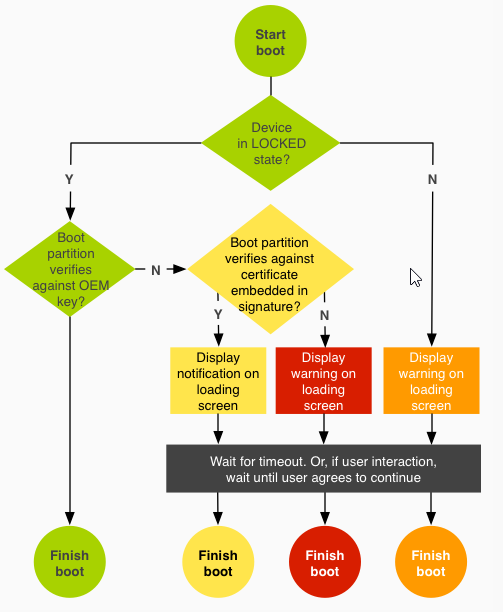
\includegraphics[width=0.7\linewidth, height=0.5\textheight]{android_pages/graphics/VerifiedBoot}
		\caption[Verified boot flow\protect\cite{VerifyingBoot}]{Verified boot flow\protect\cite{VerifyingBoot}}
		\label{fig:VerifiedBoot}
	\end{figure}
	
\begin{flushleft}
	Mit diesem Vorgehen wird auch die Integrität des Kernels sichergestellt, der in der \textit{/boot-} Partition abgelegt ist. Die Steuerung wird nach diesem Vorgang an den Kernel übergeben, welcher die Verifikation weiterer Partitionen übernimmt.\newline\\

	Um zu verhindern, dass Angreifer einfach den Bootloader manipulieren um an Daten heranzukommen, muss die Partition welche die Nutzerdaten beinhaltet (\textit{/userdata}) vor einer Veränderung an dem Bootsystem formatiert werden.
\end{flushleft}
	
	\paragraph{Integritätscheck mittels dm-verity}
	Weitere Integritätschecks werden von der Kernelfunktion dm-verity übernommen.
	dm-verity arbeitet mit einem SHA-256 Hash-tree, der wie folgt aufgebaut ist:\\
	Für jeden 4K Sektor auf der Partition wird ein Hashwert berechnet. Jeweils \textit{n} dieser Werte werden wiederum zu einem Neuen verrechnet, wobei \textit{n} ein Parameter für diese Funktion ist und während der Implementierung festgelegt wird. Dies wird solange wiederholt, bis nur noch ein Hashwert, der \textit{root-hash}, übrig ist. Zur Sicherstellung der Integrität wird dieser root-hash, mit einem bereits berechneten Soll-Wert verglichen. Sind diese identisch, ist die Partition integer.
	
	\begin{figure}[h]
		\centering
		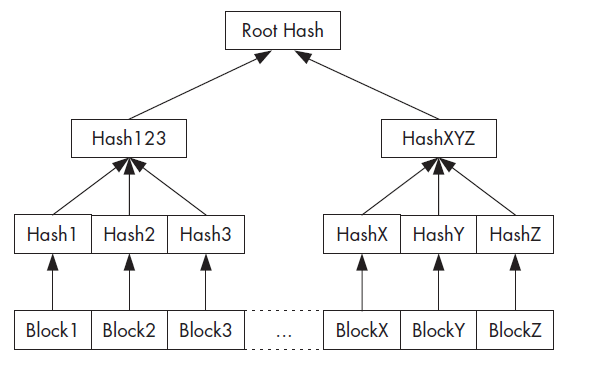
\includegraphics[width=0.7\linewidth]{android_pages/graphics/dm_verity_hash_tree.png}
		\caption[Aufbau des Hash-Trees]{Aufbau des von dm-verity erstellten Hash-Trees \protect\cite[S. 255]{Drake2014}}
		\label{fig:dm-verity-table}
	\end{figure}
	
\begin{flushleft}
	Um Manipulationen am Soll-Wert zu unterbinden, wird der Hash-Tree und ein Salt mit einem RSA Schlüssel signiert. Der genutzte RSA Public Key wird in der Boot-Partition abgelegt \cite[S. 255]{Drake2014}. Der Hash-Tree und der Salt hingegen werden hinter dem letzten Datenblock auf die zu verifizierenden Partitionen geschrieben. Besonders geeignet ist dieses Verfahren für Read-Only Partitionen, wie die System-Partition (\textit{/system}), welche das Betriebssystem beherbergt.\\
	Welche Partitionen mittels dm-verity auf ihre Integrität überprüft werden sollen, wird über einen Eintrag zu der jeweiligen Partition in der fstab-Datei festgelegt.
\end{flushleft}

	\subsubsection{Basis Rechtesystem}\label{sec:BasisRechteSystem}
	Von Linux wurde auch das Basis-Rechtesystem übernommen, allerdings wird es leicht abgewandelt genutzt. Anstatt das ein Nutzer - im Sinne von der Person, die das Gerät bedient - des Mobilsystems eine eindeutige User-ID (UID) zugewiesen bekommt, wird jede Applikation auf dem System als ein Nutzer angesehen und bekommt zur Installationszeit eine UID. Jeder Nutzer, und somit jede App, arbeitet grundsätzlich erst einmal nur innerhalb der ihm zugewiesenen Sandbox und dem damit verbundenen Dateisystem.\\\\
	Da es dennoch in vielen Fällen nötig ist, Daten zwischen verschiedenen Apps auszutauschen, gibt es mehrere Wege dies zu tun. Die üblichen Wege wären Intends oder Contentprovider. Zusätzlich gibt es noch die Möglichkeit mehreren Apps dieselbe UID zuweisen zu lassen. Allerdings ist das nur möglich, wenn die entsprechenden Applikationen mit dem selben Zertifikat signiert wurden und in deren Manifest Datei eine gemeinsame UID festgelegt wurde.
	Mittlerweile bieten die meisten Android Geräte auch einen Multiuser-Betrieb an. Da ein Linux-Nutzer eine oder mehrere Apps darstellt, wird, um zwischen verschiedenen Endnutzern zu unterscheiden, an die UID der Apps für jeden Endnutzer noch ein Prä- oder Suffix der den physikalischen Nutzer identifiziert hinzugefügt.\\\\
	Durch dieses Vorgehen bekommt jede Applikation ihren eigenen Speicherbereich, der nur für diese zugänglich ist. Durch dieses Rechtesystem wird versucht sicherzustellen, dass kein Nutzerprogramm als \textit{root} ausgeführt wird \cite[Kapitel Android's Security Model  - Application Sandboxing]{Drake2014}.
	
	\subsubsection{SELinx in Android}
	Das \textit{Discretionary Access Control (DAC)} System des Linux Kernels lässt nur relativ grobe Einstellungen zu. Hat man beispielsweiße eine Applikation, die höhere Rechte für die Ausführung benötigt, so bekommt diese unter Nutzung von DAC oftmals noch zusätzliche Rechte, welche die App nicht haben sollte.	Um dieses Problem zu beheben wird seit Android 4.4 zusätzlich zum DAC noch SELinux und dessen \textit{Mandatory Access Control (MAC)} System genutzt.
	\begin{quote}
	SELinux operates on the ethos of default denial. Anything that is not explicitly allowed is denied. \cite{SELinuxAndroid}
	\end{quote}
\begin{flushleft}
	Dabei wird, nur sofern das DAC System einen Zugriff gewährt, das MAC System konsultiert. Welche Rechte eine Applikation hat und welche nicht, wird unter SELinux in MAC Policies festgehalten.\\
	
	Es sind zwei Nutzungsmodi zu unterscheiden. Während im \textit{permissive mode} Regelverstöße nur geloggt werden, wird im \textit{enforcing mode} die strikte Einhaltung erzwungen. In den Versionen 4.3 bis exklusive 5.0 war der \textit{enforcing mode} nicht überall in Nutzung. Dies änderte sich mit Version 5.0. Seitdem läuft nur noch dieser Modus \cite{SELinuxAndroid}.
\end{flushleft}
	
	
	
	